\chapter{Dataset}
In this chapter we will describe in detail, what simulations did we run and and what we found was the best strategy to do the automated temperature fitting. In the last section, we dive discuss the dataset obtained by temperature fitting.
\section{EPOCH Simulations}
The EPOCH simulation was run in following setting:
\begin{itemize}
	\item The laser wavelength is 1 micron.
	\item The laser is p-polarized and focused to a Gaussian spot of size $3.2$ mircons.
	\item The density in the target ranges from about $0.01n_c$ to $3.\gamma_{osc}n_c$, where $n_c$ is critical density of laser radiation \cite{cui2013} and $\gamma_{osc}$ is defined in \cite{cui2013}.
	\item The initial temperature of plasma is 100 eV.
	\item The target is composed of electrons and protons. They are represented by 30 macro-particles per cell.
	\item They are represented by 30 macro-particles per cell. The resolution of spatial grid is 33nm and the time step satisfies the CFL condition \cite{arber2015}.
	\item The intensities of the laser: $I=10^{17}\,\mathrm{W.cm}^{-2}$, $I=10^{18} \,\mathrm{W.cm}^{-2}$ and \newline$I=10^{19}\,\mathrm{W.cm}^{-2}$.
	\item The angle of incidence with respect to target normal direction: \newline $\alpha \in \{0\degree,1\degree,2\degree,3\degree,4\degree,5\degree,10\degree,20\degree,30\degree,40\degree,45\degree,50\degree,60\degree\}$.
	\item The characteristic scale length of the preplasma: \newline $L\in\{0.01,0.02,0.05,0.1,0.2,0.5,1,2,5\}$ in microns.
	
\end{itemize}
The simulations have been performed on the Q3 node of the Quantum Hyperion cluster at FNSPE. The input file that used to start the EPOCH simulation can be seen in appendix \ref{att:input-deck}.

\section{Temperature fitting}
The results of the simulations are transformed into histograms as it was described in the beginning of chapter \ref{ch:temp-fitting-theory}. We fixed the energy histogram size to 1000 bins with their width scaling with the maximum electron energy. In several following pages, we will describe a strategy we developed and used to find the temperature from the vast majority of the energy histograms. The effectiveness of this strategy varies for different histograms, because it depends on multiple properties.

To get the best possible hot electron temperature fit, three things are important. First, because of the imperfections of the histogram related to the beginning and the end of the energy spectrum, it is helpful to narrow down the fitted region. Secondly, it is still necessary to perform a good fit automatically ideally without many issues. Last but not least, the fitting strategy has to be able to deal with the fact that the energy range and temperatures can for different histograms from the same dataset vary by several orders of magnitude. We will now present the strategy developed for the purpose of this thesis.


\subsection*{Fitting strategy}
Before fitting the data, it is essential to prepare it appropriately. In practice, this involves removing a few bins in the beginning of the electron energy spectrum. The lower energy bins can be removed, because  they can be empty or at least be affected by error, as the low energy electrons need more time to reach the virtual detector and the simulation can end before that happens. This is usually the case for histograms from simulations with lower laser intensity. Also, we made an approximation by considering Boltzmann distribution which does not work for small energies very well. Cutting the beginning is therefore justified. 

We also cut the end of the spectrum for reasons discussed in chapter \ref{ch:temp-fitting-theory}. We cut it in a place where there is a first empty bin. Apart from the main reason, it is also not practical to work with empty bins in the logarithmically transformed version of the histogram. In special cases, it might be possible to work with histograms cut with less strict approach. However, these cut-offs help the analysis to focus on the relevant parts of the spectrum.


\begin{figure}[h]
	\centering
	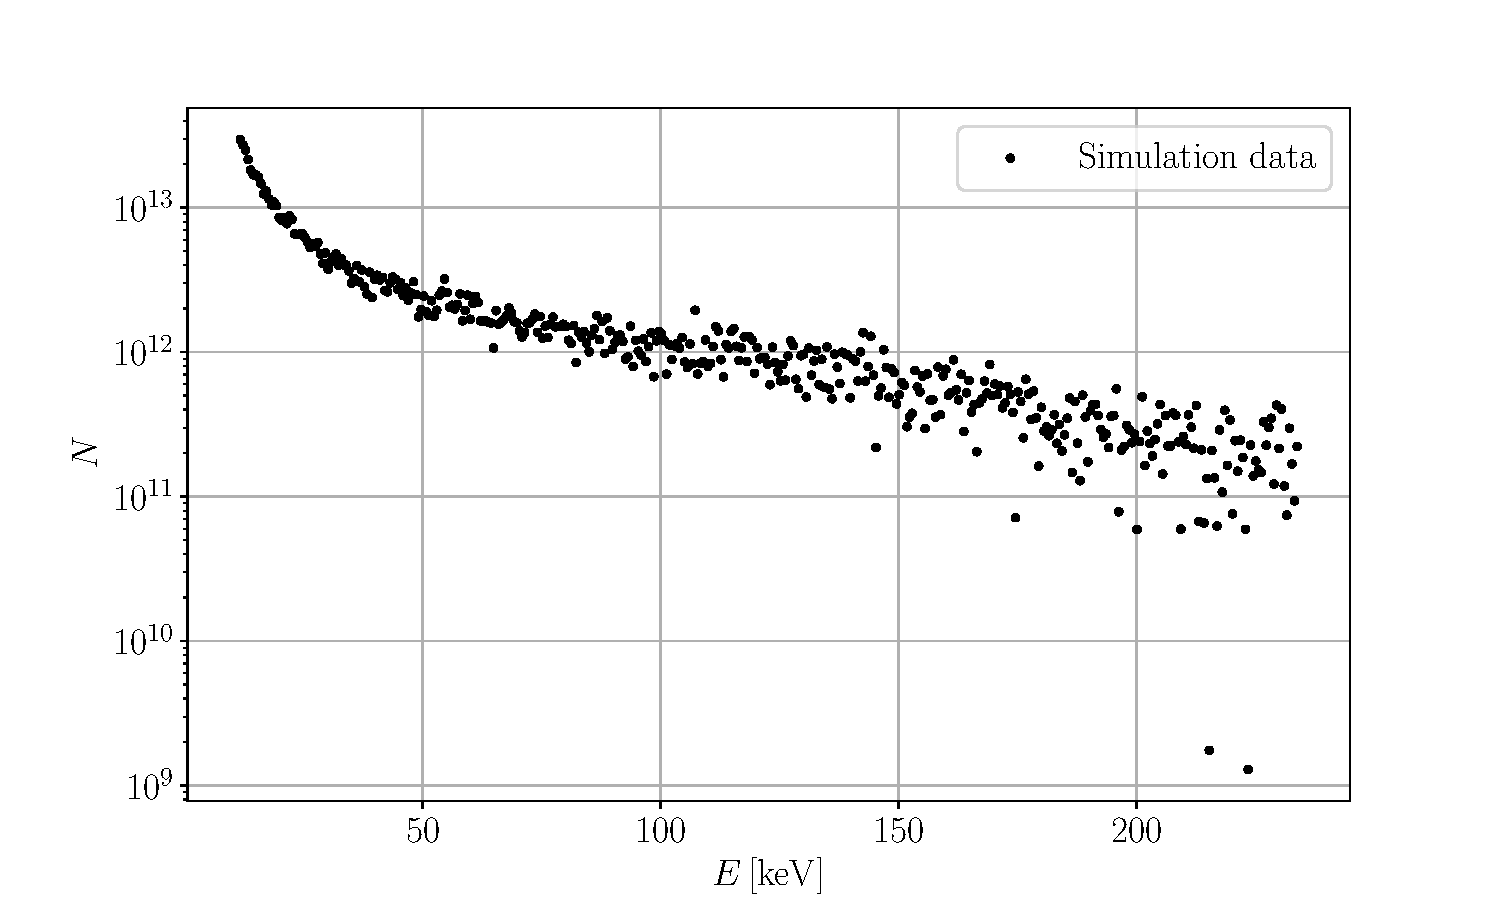
\includegraphics[width=0.9\textwidth]{figures/trimmed-hist}
	\caption{An example of trimmed histogram with simulation parameters $I=10^{19}\,\mathrm{W.cm}^{-2}$, $L=0.1\,\mathrm{\mu m}$ and $\alpha = 10$°.}
	\label{fig:trimmed-hist}
\end{figure}

The result of the cut-off of histogram \ref{fig:example-histogram} can be seen in figure \ref{fig:trimmed-hist}. Notice that the data show non-symmetrical noise in the part of the spectrum with the highest energies. This can be attributed to the logarithmic scale which can skew and seemingly magnify the noise for lower electron counts. 

For the purpose of the fitting, it is suitable to approximate the histogram data as points with $x$ values equal to the centre of the corresponding histogram bin and $y$ value equal to count.

The Jacquelin method was implemented in Python programming language as a class with number of exponential terms as a parameter. However, the lack of the numerical stability for more exponential terms usually causes issues for more than three terms because of reasons discussed at the end of chapter \ref{ch:temp-fitting-theory}. One can also choose whether the constant term should be included.

As mentioned previously, the distributions other than the hot electron distribution are not of primary concern. It is reasonable to assume that the quality of the fit improves if the fitted region is minimized, provided it still encompasses the section dominated by hot electrons. By definition, in an ideal case where the region is selected perfectly, the fit would be influenced only by noise and the other distributions, which decrease exponentially much faster as $E$ increases.

That being said, the next step aims to cut (or rather ignore) the beginning histogram once more, but now in a more sophisticated way. We found, that the majority of the histograms can be fit by the three-exponential Jacquelin method without the constant term. Of the three, there is one exponential distribution dominant for small energies. The corresponding electron distribution temperature is the lowest of all three distributions. Even though some histograms do not have three distributions present, the fit usually does not fail and the lowest temperature distribution can be (roughly) identified. We can quantify the energy $E_{\mathrm{crit}}$ at which the two most dominant terms are equal using equation:
\begin{equation}
	E_{\mathrm{crit}} = \frac{\ln{\left(a_1/a_2\right)}}{b_2-b_1}
\end{equation}
and use it as threshold for the cut-off. 

The basic illustration of the idea we just described can be seen in figure \ref{fig:3exp-fit-cut-example}. Note that $E_{\mathrm{crit}}$ intersects the fitted curve approximately in the middle of the arc where one exponential term is equal to the other. To make the lowest temperature electron distribution insignificant, the cut-off is made even a little further right. The hot electron temperature $T_\mathrm{hot}$ in figure \ref{fig:3exp-fit-cut-example} calculated by:
\begin{equation}
	T_{\mathrm{hot}} = -\frac{1}{b_3},
\end{equation}
where $b_3$ is the highest negative exponential coefficient of the whole fit. The attribute \textit{negative} is emphasized for practical reasons, because it is not guaranteed that all coefficients are. To be more precise, in some fits, the absolute value of one of the factors $a_i$ $(i=1..3)$ is small. Then the corresponding $b_i$ can be positive without significant impact on the fitted section of the histogram. In the limit of energy going to infinity, this does not have a valid physical interpretation, but in this intermediate step that does not have to bother us. In the other cases of the fit failing altogether, it often helps to narrow down the energy range even more from both ends (e.g. by 5 to 10 bins from each side) and try it again. If that fails enough times there will be nothing left and one should rather fit it differently.
	
\begin{figure}[t]
	\centering
	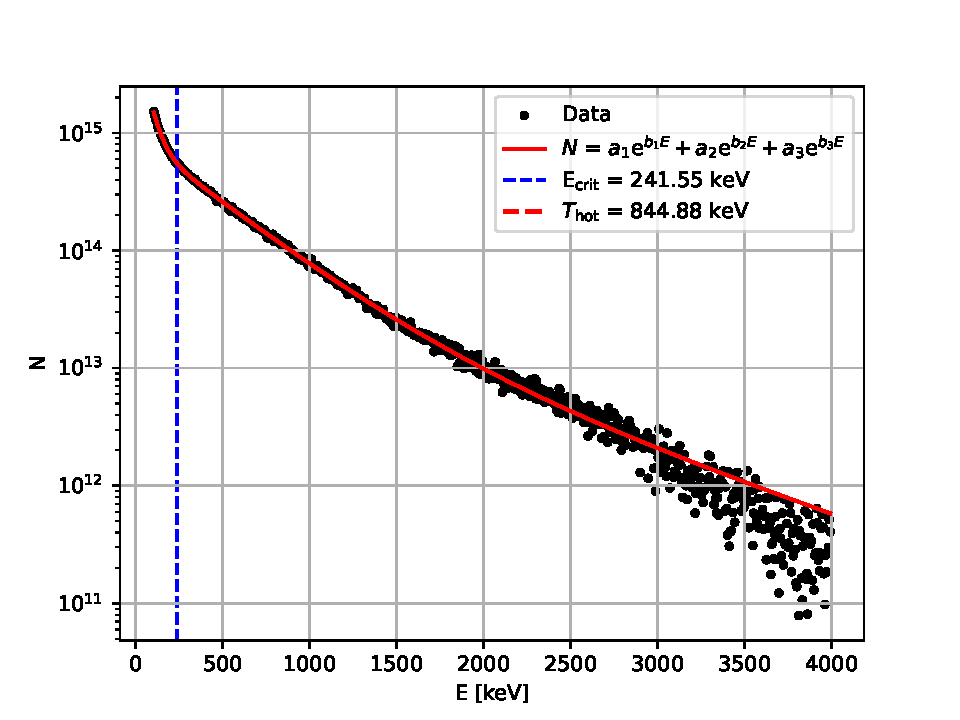
\includegraphics[width=0.9\textwidth]{figures/hist_1e19_060_30_3exp}
	\caption{An example of histogram with simulation parameters $I=10^{19}\,\mathrm{W.cm}^{-2}$, $L=0.6\,\mathrm{\mu m}$ and $\alpha = 30$° fitted with three-exponential Jacquelin method. The energy $E_{\mathrm{crit}}$ is highlighted.}
	\label{fig:3exp-fit-cut-example}
\end{figure}

We found, that in most cases after the second cut, it is now possible to perform the two-exponential Jacquelin method. The cut-off reduced the cumulative error of the partial sums, but what is more important, it justifies the lower number of the exponential terms. From our experience, the two-exponential Jacquelin fit is generally also a little bit more stable if performed on a histogram that resembles a two-exponential distribution. 

The "removal" of the lowest temperature electron distribution we just defined is similar to \textit{successive subtraction} described in chapter \ref{ch:temp-fitting-theory} in section about fitting multi-exponential functions. Here we do a similar step but from the opposite end.

The two exponential fit performed on the cut version of the histogram in figure \ref{fig:3exp-fit-cut-example} with the cut-off part plotted but not fitted is shown in figure \ref{fig:2exp-fit-example}. It is possible to see that $T_{\mathrm{hot}}$ estimate is lower than it was before. Whether two-exponential Jacquelin method on cut histogram provides better $T_{\mathrm{hot}}$ estimates compared to three-exponential Jacquelin method on the original histogram will be a part of a discussion at the end of this section. The estimate of the standard error of $T_{\mathrm{hot}}$ is calculated as:
\begin{equation}
	\label{eq:t-hot-error}
	\Delta T_\mathrm{hot} = \frac{\Delta b}{b^2} = T_\mathrm{hot}^2\Delta b,
\end{equation}
where $b$ is the corresponding exponential coefficient and $\Delta b$ is its standard deviation calculated using equation \ref{eq:b-coef-error1} or \ref{eq:b-coef-error2}.

\begin{figure}[t]
	\centering
	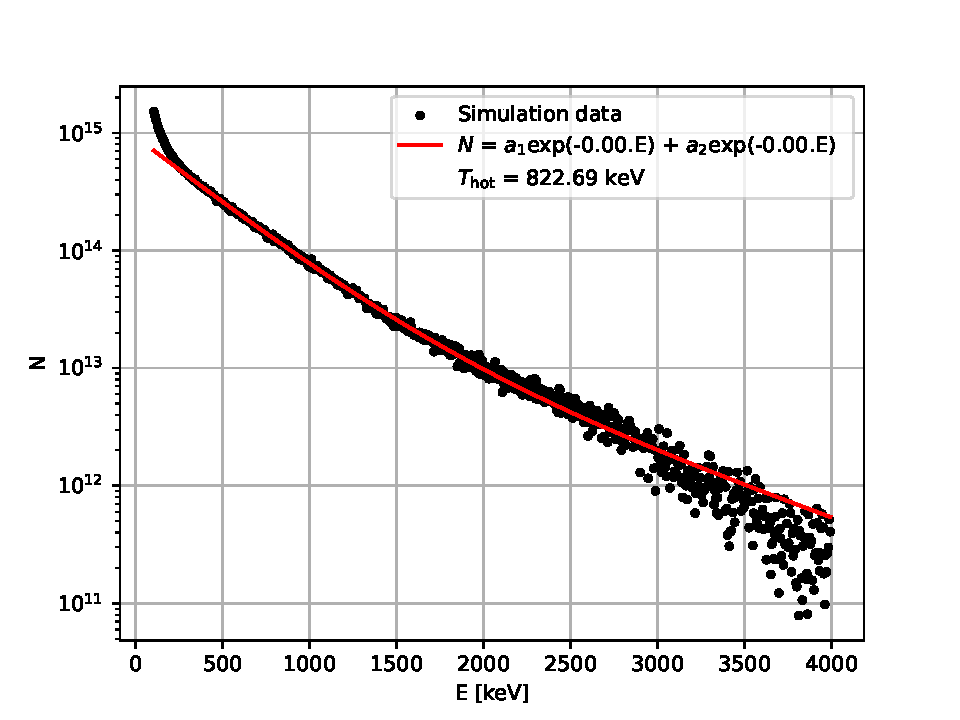
\includegraphics[width=0.9\textwidth]{figures/hist_1e19_060_30_2exp}
	\caption{An example of histogram with simulation parameters $I=10^{19}\,\mathrm{W.cm}^{-2}$, $L=0.6\,\mathrm{\mu m}$ and $\alpha = 30$° fitted with two-exponential Jacquelin method.}
	\label{fig:2exp-fit-example}
\end{figure}

As the last step of our strategy, we now use an non-linear least squares (NLSQ) algorithm to find a fit using the last result as the initial guess. It can be argued that this step is not truly necessary, because we do not have a good reason to assume that the ill-conditioning of this problem disappeared by a few cuts. However, we found, that it many cases the good initial guess provided by the explicit Jacquelin method can guide the optimizer to find a better solution. 

In general, this technique is prone to failing as it is iterative and the convergence is not guaranteed. In either case, it provides an additional insight to the quality of the fit and with . The example of the histogram from figure \ref{fig:2exp-fit-example} fitted with iterative non-linear square method using \textit{scipy.optimize.curve\_fit} function in Python can be seen in figure \ref{fig:nlsq-fit-example}.
\begin{figure}[t]
	\centering
	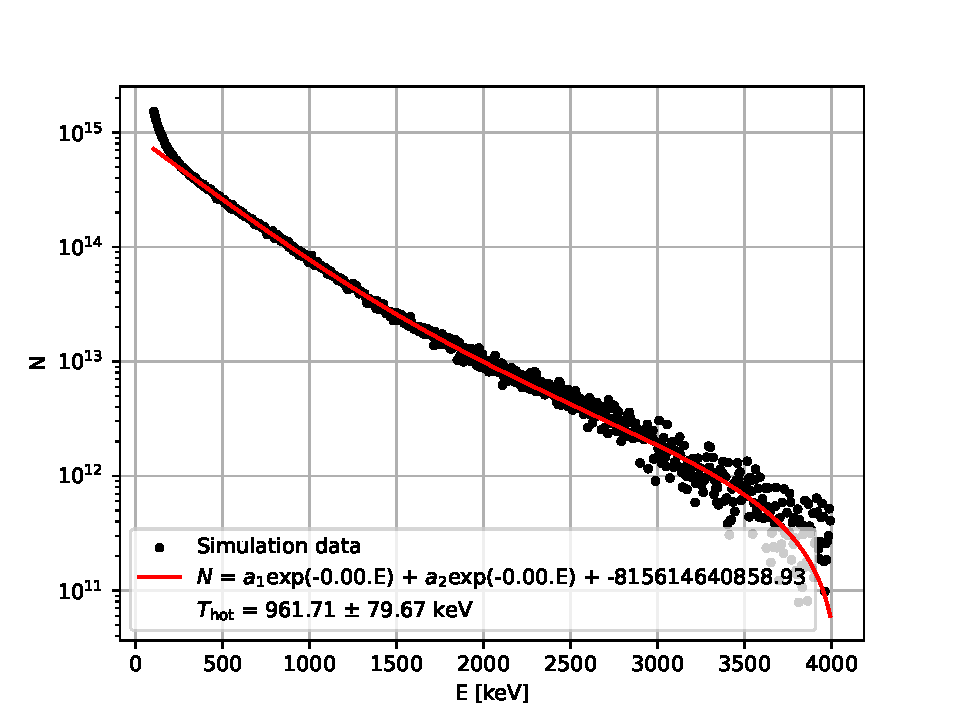
\includegraphics[width=0.9\textwidth]{figures/hist_1e19_060_30_nlsq}
	\caption{An example of histogram with simulation parameters $I=10^{19}\,\mathrm{W.cm}^{-2}$, $L=0.6\,\mathrm{\mu m}$ and $\alpha = 30$° fitted with weighted non-linear least-squares.}
	\label{fig:nlsq-fit-example}
\end{figure}

This was the last step of our strategy. We will discuss how the quality of the intermediate $T_{\mathrm{hot}}$ estimates changes with each step. The comparison is done with respect to \textit{manually} fitted histograms. \textit{Manually} means, that we select the region where distribution of hot electron dominates and perform one-exponential fit. We use an iterative weighted NLSQ method using coefficients from linear regression as initial guess. It is true, that the selection is subjective, but as of now, it is the most reliable way of finding the hot electron temperature.

As we said in the chapter \ref{ch:temp-fitting-theory}, a tool was developed to make the manual fitting of $T_{\mathrm{hot}}$ more effective. The effectiveness has roots in the possibility to load the whole folder with histograms and for each select the most reasonable region with two clicks of the mouse. The tool was developed in Python using PyQt6 framework.

There is no need to show the functionality of the tool in detail. It is basic tool tailored to make the fitting easier while also working automatically creating the dataset. We are also using custom format to save the dataset so it might be in the future extended to support different fitting strategies. Currently the only option is to select the range and click "Fit". The tool also provides an option to show the original fit obtained by automated process. 

Example of a fit performed manually can be seen in the figure \ref{fig:manual-fit-example}. First thing to notice is the selected region. In this example it is quite narrow, but maybe it could have been maybe a little wider while still only enclosing the right region. Other than that, it is now clear that the automated fit of temperature is in this series of examples off by a big margin despite the fit the figure \ref{fig:nlsq-fit-example} is seemingly behaving well.

\begin{figure}[t]
	\centering
	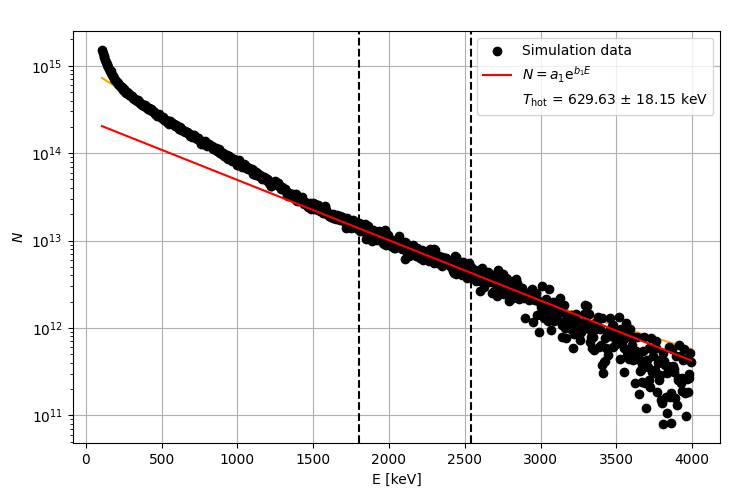
\includegraphics[width=0.9\textwidth]{figures/hist_1e19_060_30_manual}
	\caption{An example of histogram with simulation parameters $I=10^{19}\,\mathrm{W.cm}^{-2}$, $L=0.6\,\mathrm{\mu m}$ and $\alpha = 30$° fitted manually with the fitting tool.}
	\label{fig:manual-fit-example}
\end{figure}

Quantitative analysis of the fitting strategy and its $T_\mathrm{hot}$ estimates will be done in the following way. For each histogram for which the NLSQ method converged (359 out of total 373), we take all three $T_\mathrm{hot}$ estimates of 3-exponential method $T_\mathrm{hot,3exp}$, 2-exponential method $T_\mathrm{hot,2exp}$ and NLSQ estimate $T_\mathrm{hot,NLSQ}$ and calculate their relative error to the manual fit estimate $T_\mathrm{hot,manual}$ using:

\begin{equation}
	\mathrm{Relative \, error} = \frac{T_\mathrm{hot,2exp}-T_\mathrm{hot,manual}}{T_\mathrm{hot,manual}}
\end{equation}

and for $T_\mathrm{hot,NLSQ}$ and $T_\mathrm{hot,3exp}$ analogously. A comparison of mean square relative error for all three steps of the strategy is shown in Table \ref{tab:means_mses}. From this table, it is evident that in general it can be said that the fit improves during the strategy, because the relative error is most likely better for NLSQ than for 2-exponential fit.  

\begin{table}[ht]
	\centering
	\begin{tabular}{lc}
		\toprule
		Method & MSRE \\
		\midrule
		3exp  & 16.61 \\
		2exp  & 0.32 \\
		NLSQ & 0.06 \\
		\bottomrule
	\end{tabular}
	\caption{Mean Squared Relative Errors for fitting methods.}
	\label{tab:means_mses}
\end{table}


We plot the relative errors with respect to $T_\mathrm{hot,manual}$ for each evaluated simulation. The scatter plot containing the relative errors can be seen in the figure \ref{fig:relative-errors}. We are not plotting the 3-exp results. From this graph, we can conclude that the majority of the $T_\mathrm{hot}$ estimates is within the relative error of 0.5. That is probably acceptable for small values of $T_\mathrm{hot}$ (up to 20 keV), because the absolute value of this error is not significant. For higher energies, having relative error 0.5 is disappointing to say the least, but it again points to the fact that the automation of the fitting is very challenging.

\begin{figure}[ht]
	\centering
	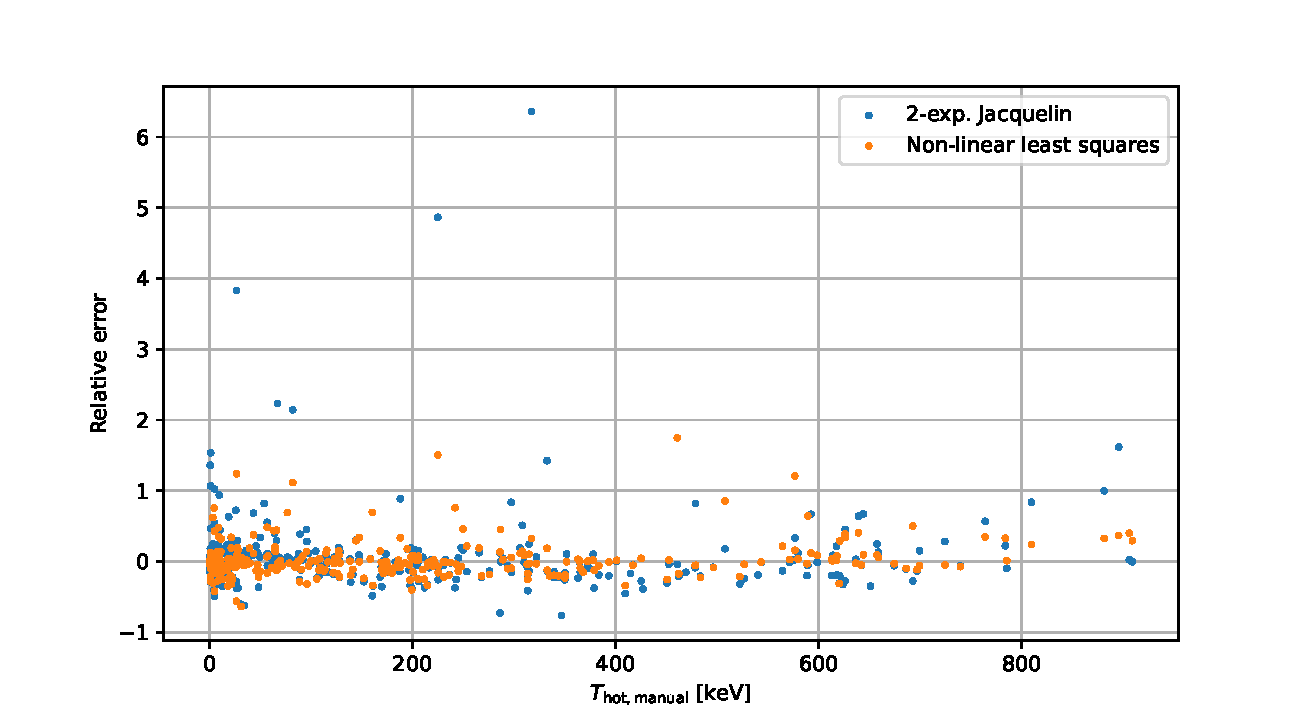
\includegraphics[width=0.98\textwidth]{figures/relative-error}
	\caption{Relative errors of the $T_\mathrm{hot}$ for two fitting methods.}
	\label{fig:relative-errors}
\end{figure}


Despite various attempts, we were unable to make further progress from this point. One potential approach is to repeat the cut-off process. However, this introduces several complications. First, it is challenging to perform the cut-off without excessively reducing the region dominated by the $T_\mathrm{hot}$ distribution. During the initial cut-off, removing a larger portion of the second distribution is not problematic. However, in this case, it significantly impacts the results, likely because the end of the histogram does not belong to any of the distributions and therefore it is skewing the fit. Secondly, the one-exponential fit is more sensitive to data that do not belong to the fitted distribution. This sensitivity means that if the histogram is cut in a way that leaves a trace of the distribution intended to be removed, the one-exponential fit produces worse estimates of $T_\mathrm{hot}$ than the two-exponential fit.

A metric for comparing two fits of the same histogram side by side is also not trivial. Presenting such metric was one of the goals of this thesis. A comparison of the automated fits can be done by using weighted mean squared error:
\begin{equation}
	WMSE = \frac{\sum_{i=1}^{n}w_i(y_i-\bar{y}_i)^2}{\sum_{i=1}^{n}w_i}
\end{equation}
where $\bar{y}_i$ is the predicted value and $w_i$ are weights. The weights can be for instance set equal to standard deviation estimated as using Poisson statistics $\sigma_i = 1/y_i$. The idea is to compensate for the the bigger variance for smaller energies. After using our fitting strategy, this metric correctly labels 245 fits out of 359 to be better compared with respect to manually fitted value.

In conclusion, there definitely is a room for improvement of this process, if one wants to rely on fitting thousands of histograms at once. The presented strategy can produce acceptable results, but in current state it probably shouldn't be completely unsupervised. The failed fits have to be handled separately and without briefly
checking each histogram, the reliability is questionable. Needless to say, it may serve as starting point for further improvement.

\section{Full dataset}
In this section, we will present the dataset used for modelling. Naturally, the results from 378 simulations contain a lot of information most if which will be discarded. As we concluded at the end of the previous section, the automation of the temperature fitting brings many challenges, some of which were not exhaustingly solved. From now on, we will be using the manually labelled dataset as such data are considered the most reliable. The main goal of this section is to visualize the interesting aspects of the data we obtained so far.
\begin{figure}[ht]
	\centering
	\begin{subfigure}{0.49\textwidth}
		\centering
		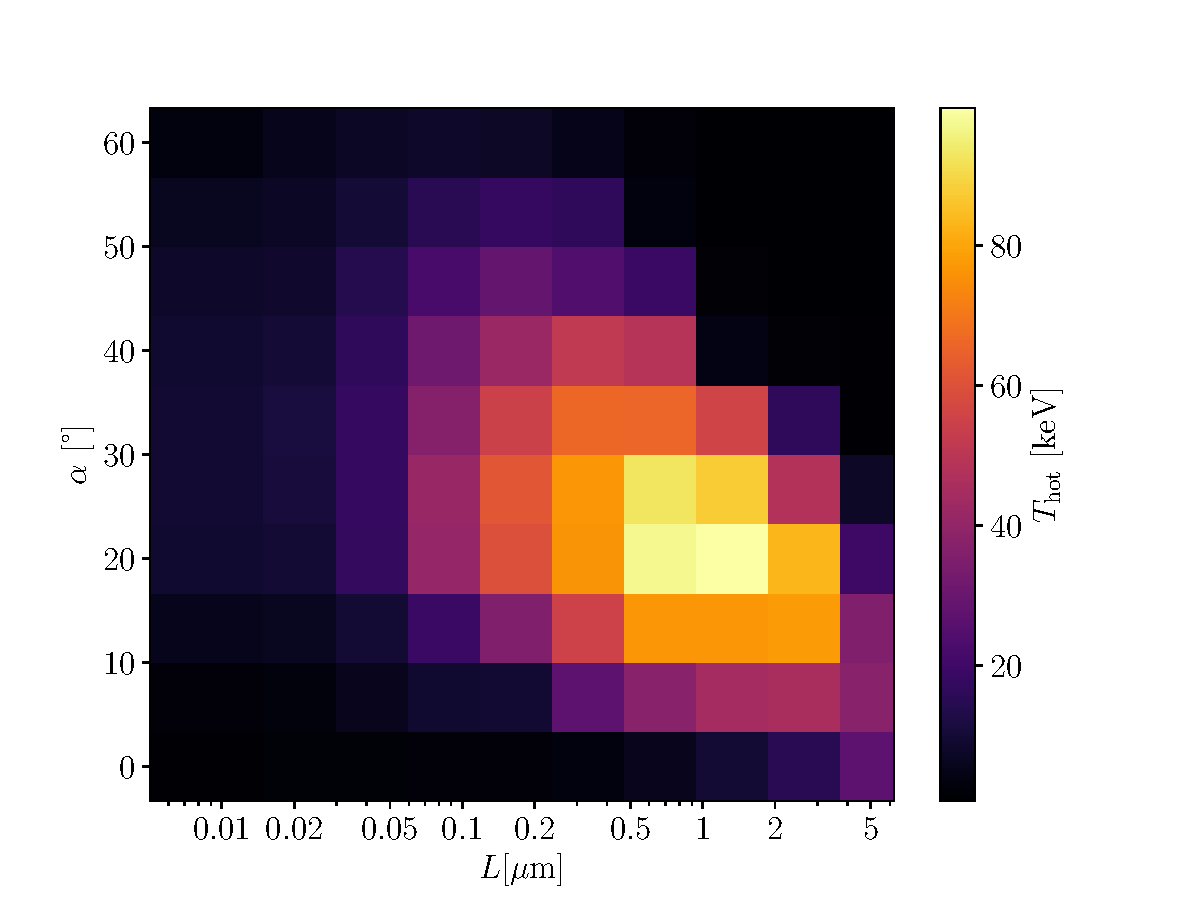
\includegraphics[width=\textwidth]{figures/I_1e17t_hot}
		\caption{Dataset with $I = 1 \times 10^{17} \mathrm{W.cm}^{-2}$.}
		\label{fig:dataset1-a}
	\end{subfigure}
	\hfill
	\begin{subfigure}{0.49\textwidth}
		\centering
		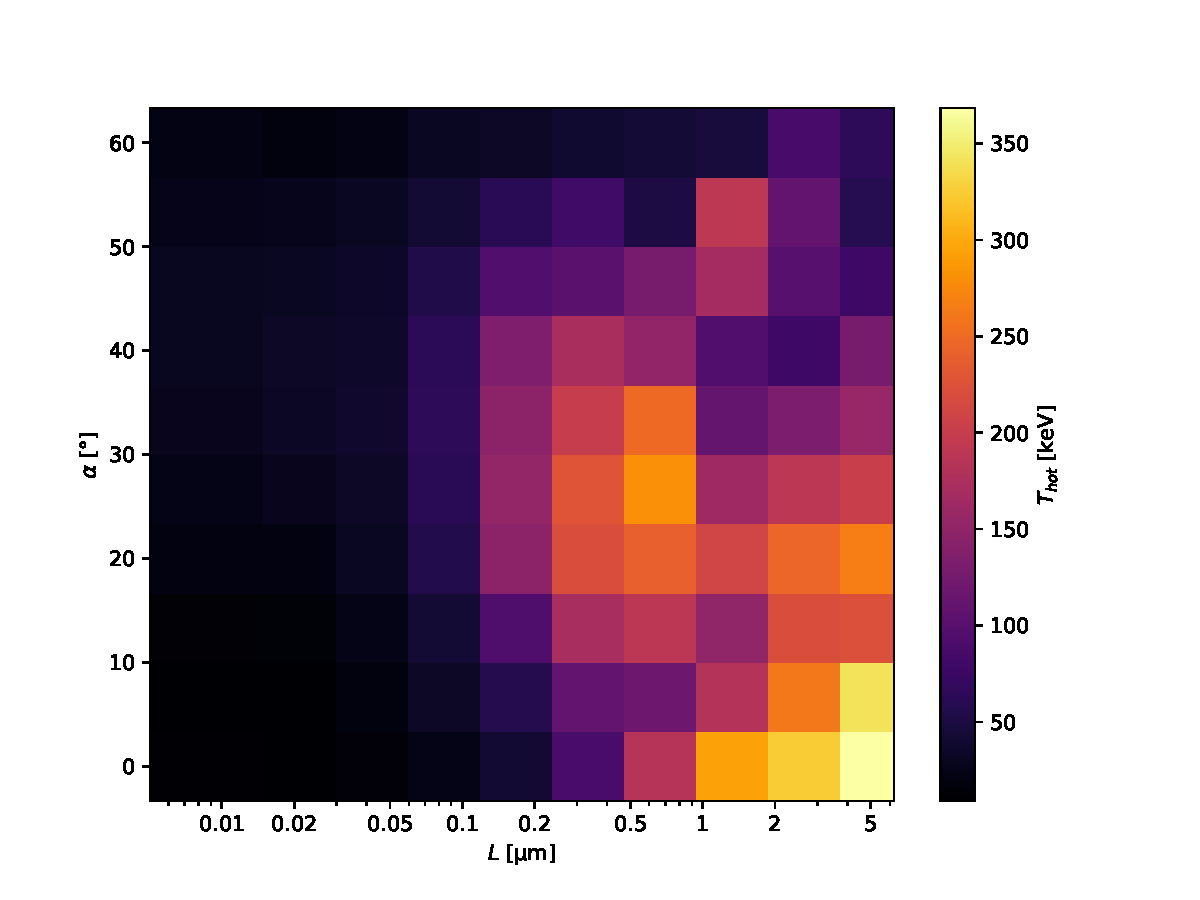
\includegraphics[width=\textwidth]{figures/I_1e18t_hot}
		\caption{Dataset with $I = 1 \times 10^{18} \mathrm{W.cm}^{-2}$.}
		\label{fig:datset1-b}
	\end{subfigure}
	\begin{subfigure}{0.49\textwidth}
		\centering
		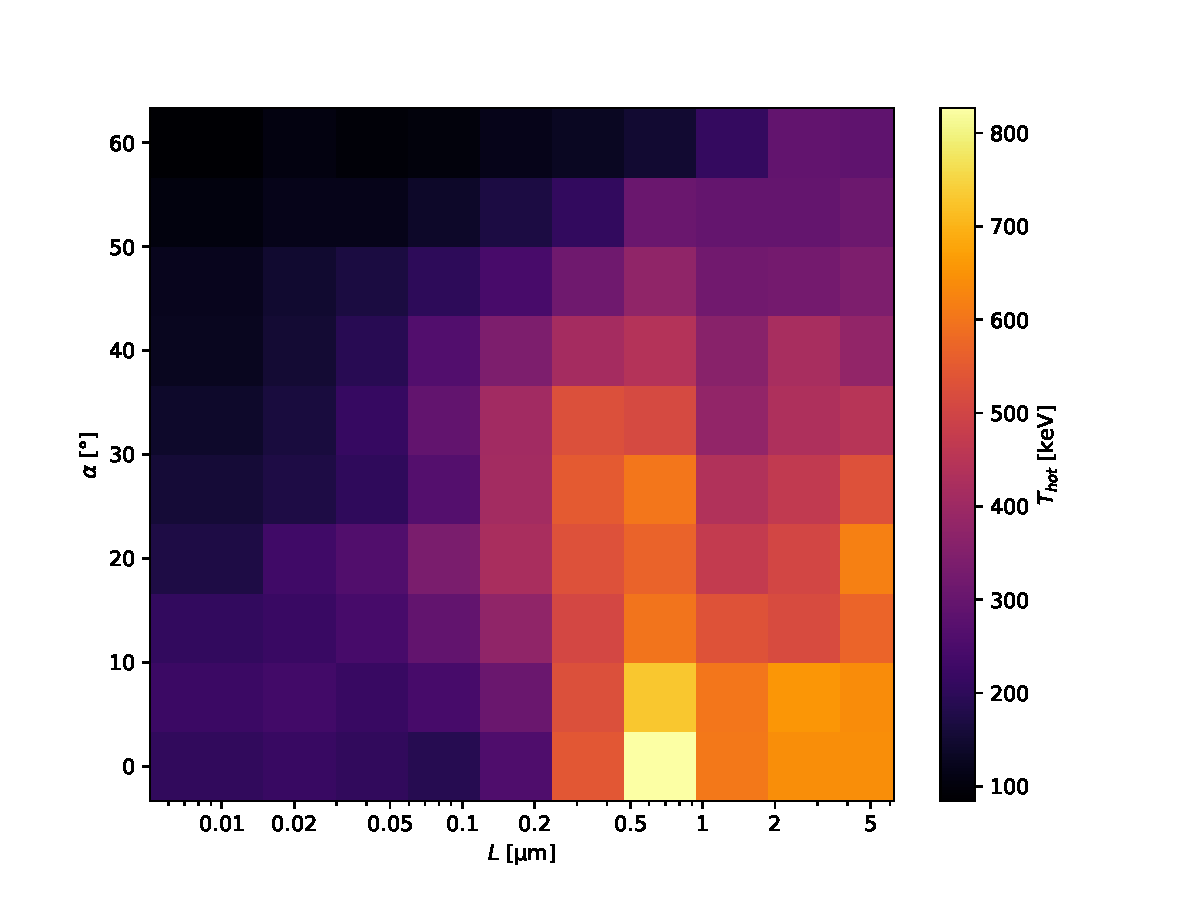
\includegraphics[width=\textwidth]{figures/I_1e19t_hot}
		\caption{Dataset with $I = 1 \times 10^{18} \mathrm{W.cm}^{-2}$.}
		\label{fig:dataset1-c}
	\end{subfigure}
	\caption{Illustration of dataset shown for three simulated intensities.}
	\label{fig:dataset1}
\end{figure}


The visualization of the dataset itself can give us valuable insight to the behaviour of the function of $T_{\mathrm{hot}} = T_{\mathrm{hot}}(I,l,\alpha)$. Because there are three quantities by which $T_{\mathrm{hot}}$ is being modelled, the visualization can be tricky. The issue can be approached from multiple points of view.

Let us start by showing the dependency of the fitted temperature on simulation parameters with three fixed intensities $I = 1 \times 10^{17} \,\mathrm{W.cm}^{-2}$, $I = 1 \times 10^{18} \,\mathrm{W.cm}^{-2}$ and $I = 1 \times 10^{19} \,\mathrm{W.cm}^{-2}$. This way we can "slice" through the three dimensional space of parameters and get a good idea what we are modelling. By the way, this approach is almost completely corresponding to the way the parameter space was sampled for the simulations. Most of the parameters were chosen as a points of grid with certain steps in $\alpha$ and logarithmic steps in $l$. This is not true for all points and because of that, these graphs were made using linear interpolation to the grid of similar density. In other words, the values should not be considered exact and the graphs serve only as illustration. The graphs can be seen in figure \ref{fig:dataset1}.


The initial observation from these three graphs can for instance be the increasing temperature scales on the right side of each graph, which corresponds to the increasing intensity. This demonstrates the fundamental relationship: as the energy carried by the laser pulse increases, the temperature of the hot electrons rises too. Next thing one might notice is that size of the temperatures range also changes with intensity. For both $I = 1 \times 10^{17} \mathrm{W.cm}^{-2}$ and $I = 1 \times 10^{18} \mathrm{W.cm}^{-2}$, there is a region (or simulation point) with electron energy close to zero. For intensity $I = 1 \times 10^{19} \mathrm{W.cm}^{-2}$ there is no such phenomenon. 

It is also possible to make some qualitative comments about the dataset in the light of the absorption theory which was briefly discussed in chapter \ref{ch:plasma-theory}. We will come back to this later.

It is important to realize, that these graphs do not represent the general absorption patterns. To compare total absorption across the domain of simulation points, it is necessary to also include the energy absorbed by the rest of the electrons. We will visualize it in similar way but instead of temperature, we look at the overall energy carried by all the electrons. This can be integrating each of the histograms. For the same reasons as in the previous section, we restrict ourselves to electron energies higher than threshold of 10 keV. The total absorbed energy for the same three intensities is displayed in the graphs in figure \ref{fig:dataset2}.

\begin{figure}[ht]
	\centering
	\begin{subfigure}{0.49\textwidth}
		\centering
		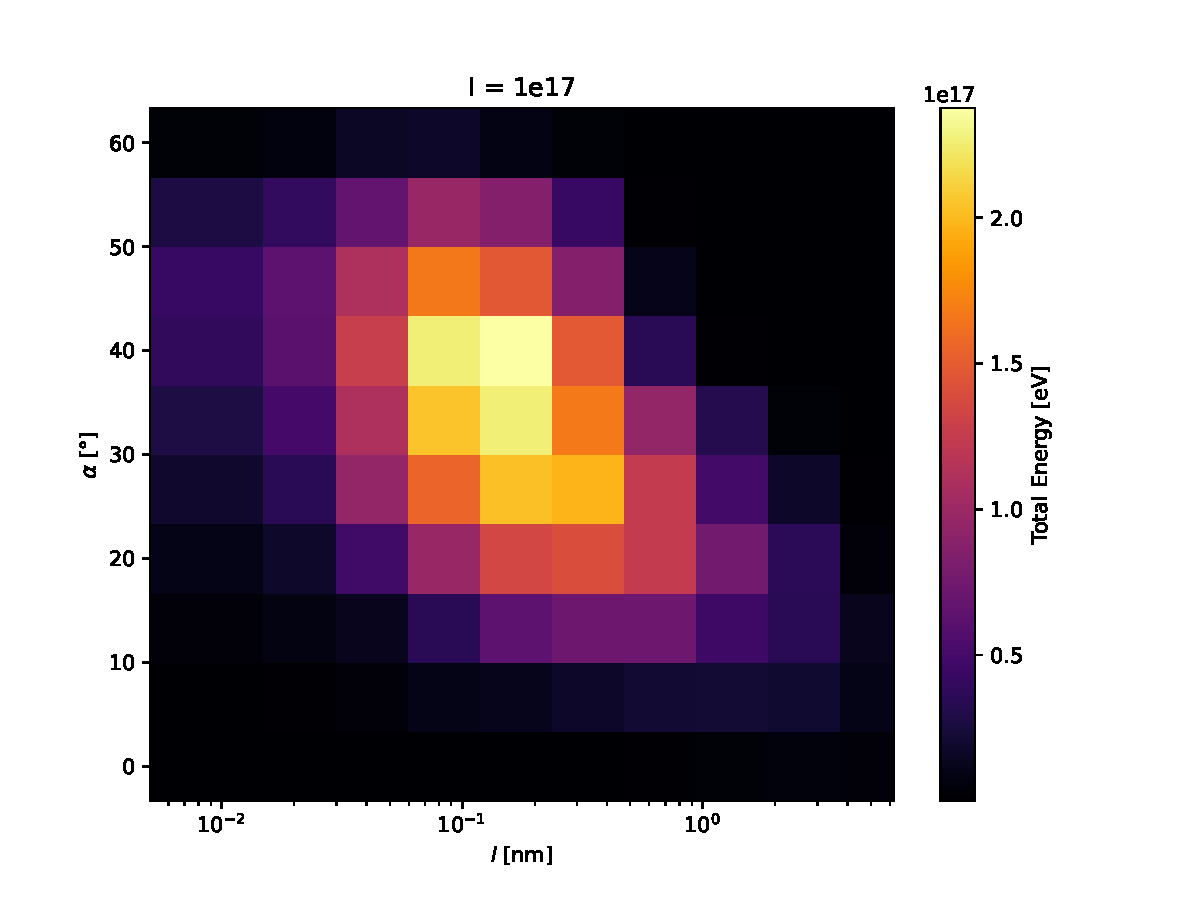
\includegraphics[width=\textwidth]{figures/I_1e17_cut_10}
		\caption{Dataset with $I = 1 \times 10^{17} \mathrm{W.cm}^{-2}$.}
		\label{fig:dataset2-a}
	\end{subfigure}
	\hfill
	\begin{subfigure}{0.49\textwidth}
		\centering
		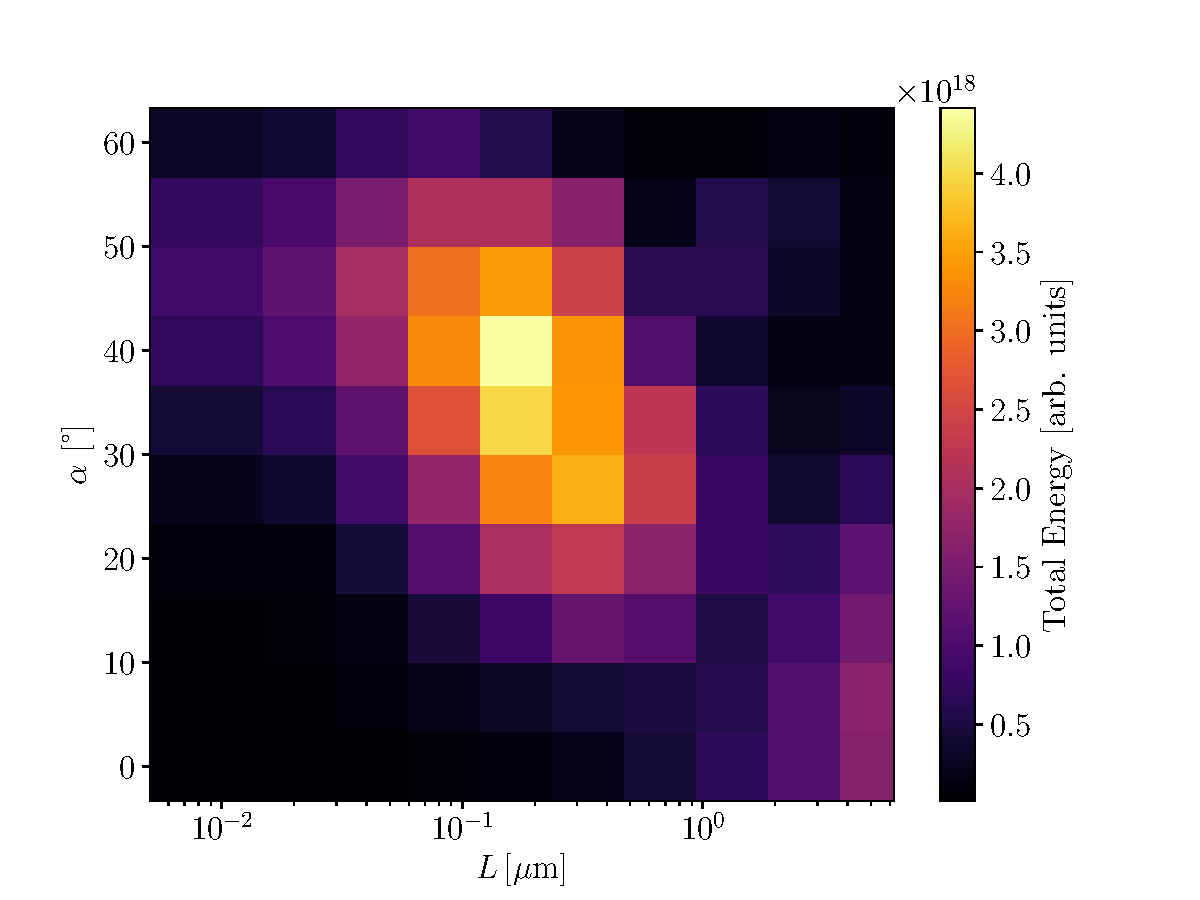
\includegraphics[width=\textwidth]{figures/I_1e18_cut_10}
		\caption{Dataset with $I = 1 \times 10^{18} \mathrm{W.cm}^{-2}$.}
		\label{fig:datset2-b}
	\end{subfigure}
	\begin{subfigure}{0.49\textwidth}
		\centering
		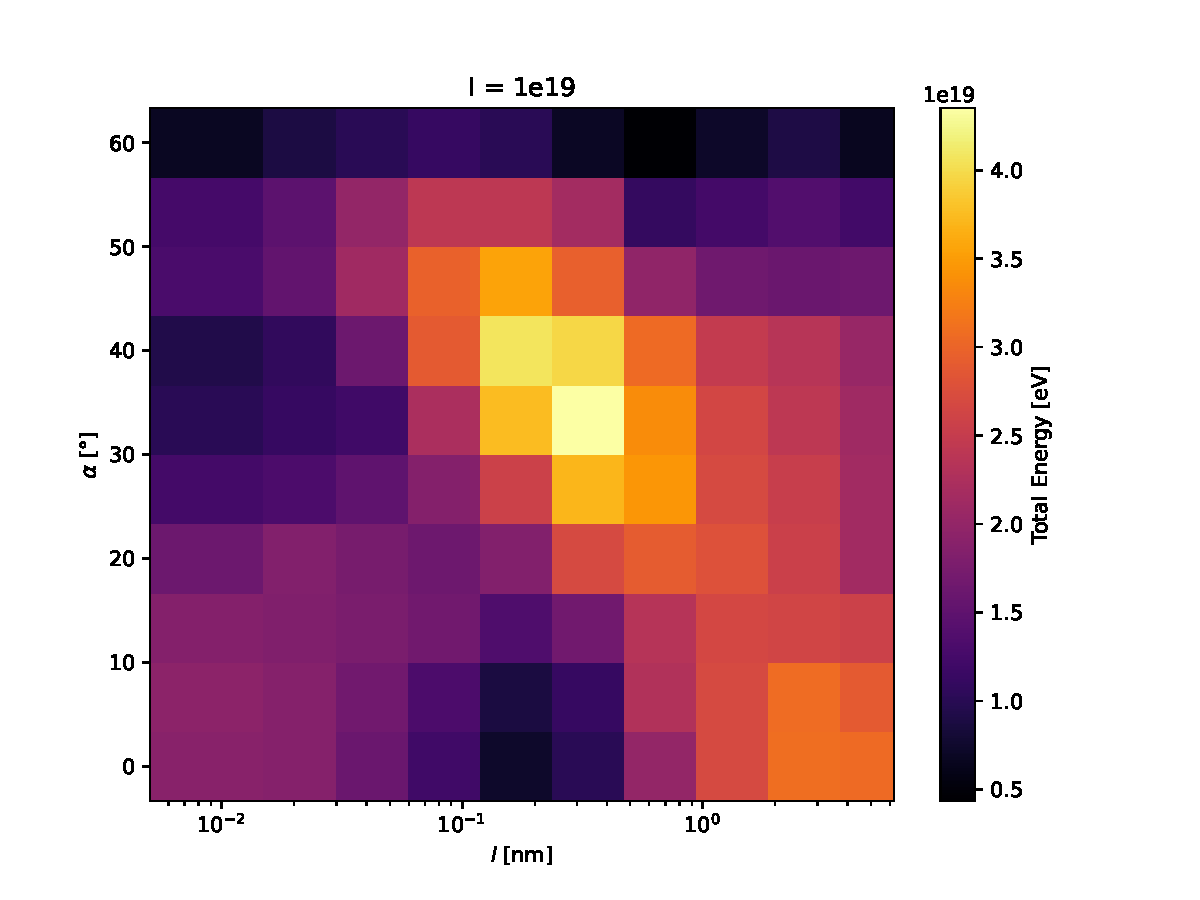
\includegraphics[width=\textwidth]{figures/I_1e19_cut_10}
		\caption{Dataset with $I = 1 \times 10^{19} \mathrm{W.cm}^{-2}$.}
		\label{fig:dataset2-c}
	\end{subfigure}
	\caption{Illustration of total energy absorption shown for three simulated intensities.}
	\label{fig:dataset2}
\end{figure}

It is possible to see, that the maximum of overall absorption is happening in cases of bigger incidence angles. This can be attributed to ???. Also for the intensity $I = 1 \times 10^{19} \mathrm{W.cm}^{-2}$ there is relatively larger absorption happening for small angles and large scale lengths. All this is in agreement with what was presented in chapter~\ref{ch:plasma-theory}.

Moving on, let us shift our attention back to the the study of the actual dataset of temperatures. Without interpolation, we can plot the temperature with respect to scale and angle of incidence so that the actual values of temperature are more clear. Three graphs corresponding to the to the same three intensities are show in the figure~\ref{fig:dataset3}.

\begin{figure}[t]
	\centering
	\begin{subfigure}{0.49\textwidth}
		\centering
		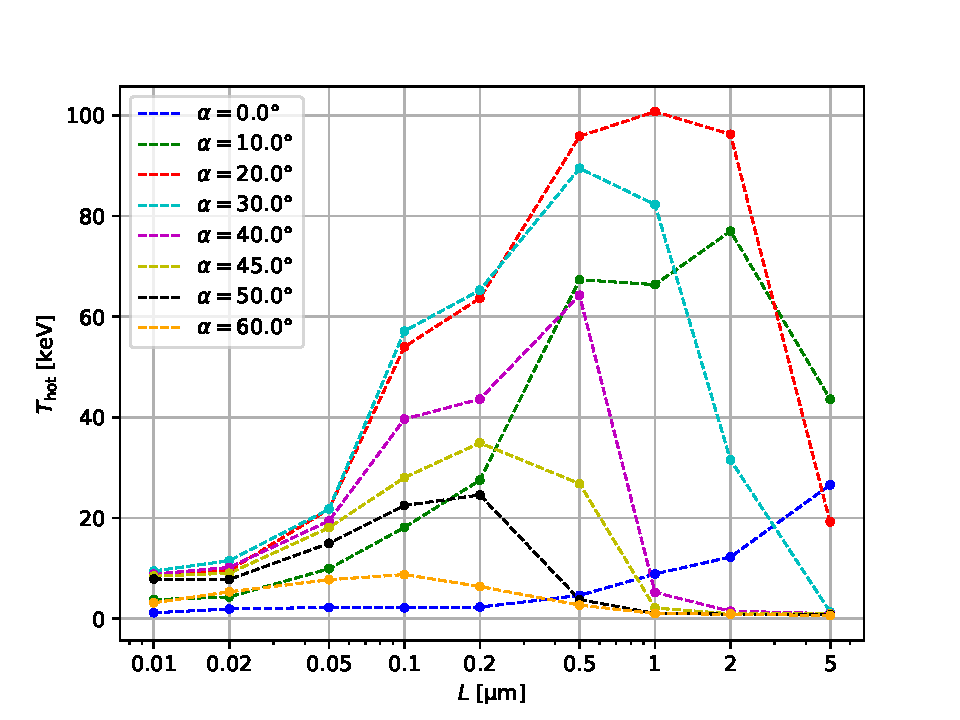
\includegraphics[width=\textwidth]{figures/t_hot_l_17}
		\caption{Dataset with $I = 1 \times 10^{17} \mathrm{W.cm}^{-2}$.}
		\label{fig:dataset3-a}
	\end{subfigure}
	\hfill
	\begin{subfigure}{0.49\textwidth}
		\centering
		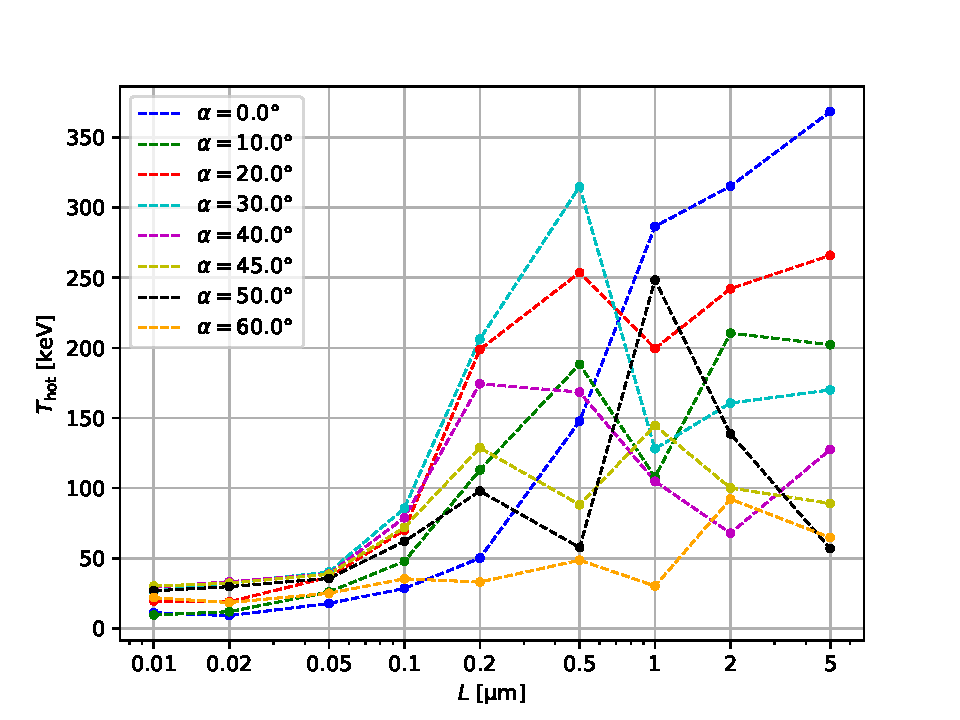
\includegraphics[width=\textwidth]{figures/t_hot_l_18}
		\caption{Dataset with $I = 1 \times 10^{18} \mathrm{W.cm}^{-2}$.}
		\label{fig:datset3-b}
	\end{subfigure}
	\begin{subfigure}{0.59\textwidth}
		\centering
		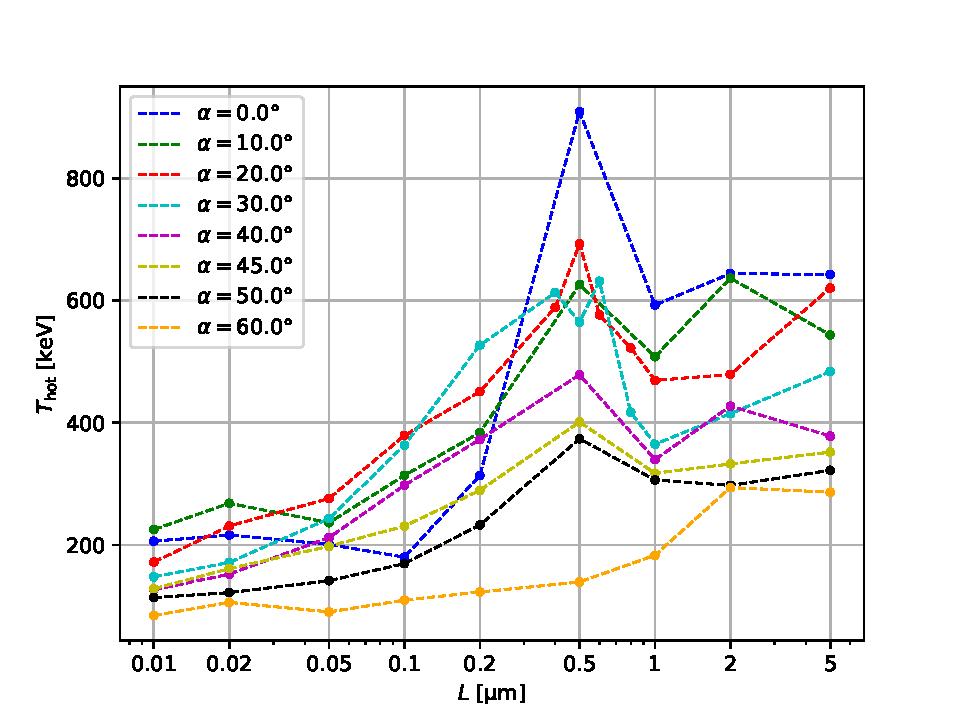
\includegraphics[width=\textwidth]{figures/t_hot_l_19}
		\caption{Dataset with $I = 1 \times 10^{19} \mathrm{W.cm}^{-2}$.}
		\label{fig:dataset3-c}
	\end{subfigure}
	\caption{Illustration of total energy absorption shown for three simulated intensities.}
	\label{fig:dataset3}
\end{figure}

Here, what might be particularly interesting is the evident rise of temperatures for $l=0.5 \mathrm{\mu m}$ for the intensity $I = 1 \times 10^{19} \mathrm{W.cm}^{-2}$, especially for small incidence angles. The total absorption is for these parameters relatively small, as can be seen in figure \ref{fig:dataset2-c}. (add explanation ???). For $l=0.5 \mathrm{\mu m}$, in  both of the smaller intensities the rise is apparent only for larger angles.